
\documentclass[12pt]{article}
% ====== minimal packages ======
\usepackage{amsmath,amssymb,amsfonts}
\usepackage{bm}
\usepackage{physics}
\usepackage{microtype}
\usepackage{tcolorbox}
\usepackage{mathtools}

% load hyperref *after* natbib
\usepackage[colorlinks=true,linkcolor=blue,citecolor=blue,urlcolor=blue]{hyperref}
\usepackage[utf8]{inputenc}
\usepackage[T1]{fontenc}
\usepackage[margin=2.2cm]{geometry}



% ==== Packages ====
\usepackage{lmodern}
\usepackage{booktabs}
\usepackage[caption=false]{subfig}
\usepackage{tikz}
\usetikzlibrary{arrows.meta,positioning,calc,fit,decorations.pathmorphing}

% swirl arrows (context-aware)
\DeclareRobustCommand{\swirlarrow}{
\mathchoice{\mkern-2mu\scriptstyle\boldsymbol{\circlearrowleft}}%
{\mkern-2mu\scriptstyle\boldsymbol{\circlearrowleft}}%
{\mkern-2mu\scriptscriptstyle\boldsymbol{\circlearrowleft}}%
{\mkern-2mu\scriptscriptstyle\boldsymbol{\circlearrowleft}}
}%
\newcommand{\Gswirl}{\mathcal{G}\swirlarrow}


\usepackage{graphicx}

\setlength{\oddsidemargin}{0.15in}
\setlength{\evensidemargin}{0.15in}
\setlength{\textwidth}{6.2in}
\setlength{\topmargin}{-0.5in}
\setlength{\textheight}{9in}


\begin{document}


\title{Rotating-Frame Unification in Swirl-String Theory:\Swirl--EMF Coupling and Vortex Nucleation}
\author{Omar Iskandarani}
\date{October 2025}

\begin{abstract}

\noindent Swirl--String Theory (SST) posits a universal incompressible condensate (the swirl medium) in which quantized vortex loops (swirl strings) represent particles and fields. In this work, we unify rotating-frame effects in the SST canon by demonstrating that time-varying \emph{swirl density} in the medium induces an electromotive response. In particular, we derive a modified Faraday's law in which changes in swirl string areal density act as a source of electric field (via a coupling constant $\Gswirl$), analogous to a time-varying magnetic flux. This rotating-frame unification suggests that inertial (gravitational) and electromagnetic phenomena share a common fluid–topological origin. We present the conceptual framework leading to this \emph{swirl--EMF coupling}, including the canonical derivation of the coupling constant $\Gswirl$. Experimental implications are then explored: a falsifiable prediction is that nucleation, reconnection, or annihilation of swirl vortices produces a quantized electromotive impulse of magnitude $\Phi_{0}$ (a flux quantum). We outline how condensed-matter systems (e.g. type-II superconductors, Bose–Einstein condensates, or magnetic defect films) can be used to simulate such topological transitions and detect the predicted quantized impulses. The conceptual novelty of this approach is highlighted, and we discuss how measuring these signals would provide empirical evidence for the SST framework or, conversely, place strong constraints on it. Technical derivations of the modified Faraday law, the vortex nucleation threshold, and impulse quantization are provided in the Appendices to maintain continuity in the main text.

\end{abstract}


\section{Introduction}

SST (Swirl--String Theory) is an emergent framework that models fundamental particles and forces as manifestations of a fictitious incompressible fluid medium \cite{Iskandarani2025Canon}. In SST, matter corresponds to quantized vortex filaments (``swirl strings'') in a universal condensate, and macroscopic forces arise from collective fluid dynamics rather than spacetime curvature. For example, previous works have shown that gravity can be interpreted as an emergent effect of coherent rotating flows in this medium \cite{Iskandarani2025RotatingFrame}. By calibrating the theory's constants, the effective gravitational coupling $\Gswirl$ in SST can be set equal to Newton's constant $G{N}$, reproducing Newtonian gravity in the appropriate limit \cite{Iskandarani2025Canon}. This picture aligns with ideas of entropic or emergent gravity \cite{Verlinde2011,Verlinde2017,Jacobson1995,Padmanabhan2010} by attributing gravitational phenomena to an underlying informational field (the swirl medium) rather than a fundamental spacetime interaction.


% [TIKZ-SUGGESTION-1: High-level schematic of SST: background ``swirl medium'' with several closed vortex loops (unknotted & knotted), arrows indicating local swirl velocity. Place near here.]


A central premise of SST is that each swirl string carries quantized circulation. In fact, the circulation of the swirl velocity field $\mathbf{v}_{\swirlarrow}$ around any closed loop $C$ is constrained to integer multiples of a fundamental quantum $\kappa$:

\begin{equation}\label{eq:circulation}

\Gamma ;=; \oint_C \mathbf{v}_{\swirlarrow}\cdot d\boldsymbol{\ell} ;=; n,\kappa, \qquad n \in \mathbb{Z},,

\end{equation}

with $\kappa$ identified as $h/m_\text{eff}$ for some characteristic mass scale $m_\text{eff}$. This postulate echoes Onsager's and Feynman's discovery of quantized vortex circulation in superfluids and is a cornerstone of the SST model \cite{Onsager1949,Feynman1955}. Topologically, swirl strings are permitted only in discrete knot or link types, such that quantum numbers (mass, charge, spin, etc.) correspond to topological invariants of the vortex filament rather than to eigenstates of quantum operators \cite{Iskandarani2025Canon}. This topological quantization gives SST a concrete combinatorial foundation distinct from field-theoretic approaches.


We follow the canonical notation established in the SST Rosetta guide \cite{Iskandarani2025Rosetta,Iskandarani2025Canon}. Important quantities include the swirl medium's mass density $\rho_{!f}$, the swirl velocity field $\mathbf{v}_{\swirlarrow}$, the core radius $r_c$ of a vortex filament (on the order of $10^{-15}$~m), and the characteristic core swirl speed $v^{\circ}$ (on the order of $10^{6}$~m/s)\footnote{Anchors the canonical numerical value/range for the vortex core radius $r_c$ used in SST.}\footnote{Anchors the canonical numerical value/range for the core swirl speed $v^{\circ}$ used in SST.}. These constants are calibrated such that SST reproduces known physical scales: for instance, $\kappa = 2\pi r_c v^{\circ}$ is chosen to yield realistic atomic energy levels, and $\Gswirl$ is set so that the emergent gravitational attraction between many swirl strings mimics Newtonian gravity at large scales \cite{Iskandarani2025Canon}. By construction, the SST canon ensures dimensional consistency and recovery of accepted limits (classical gravity, Coulomb force, etc.) in appropriate regimes\footnote{Points to the SST-canon statement that all symbols/units are dimensionally consistent.}\footnote{Points to the SST-canon guarantee of recovering accepted limits (Newton/Coulomb) in proper regimes.}.


% [TIKZ-SUGGESTION-2: Small inset illustrating the relation $\kappa=2\pi r_c v^{\circ}$ as a circle of radius $r_c$ with tangential speed $v^{\circ}$ and circulation arrows.]


The present paper extends the SST canon by demonstrating a novel unification of rotating-frame effects: we show that changes in \emph{swirl areal density} act as a direct source for electromotive force (EMF). In other words, a time-dependent distribution of swirl strings can induce electric fields in much the same way that a time-varying magnetic flux does in Faraday's law. This theoretical result, derived in Section~\ref{sec:swirlEMF}, has far-reaching implications. It suggests that the same fluid medium underlying gravity also encodes electromagnetic phenomena, effectively bridging two fundamental interactions within a single framework. The conceptual leap is to treat topological vortex dynamics (creation, annihilation, reconnection of swirl strings) as events that couple to electromagnetic fields. We will derive the modified Faraday law and identify the coupling constant $\Gswirl$ associated with this swirl–EMF interaction. Notably, we find that $\Gswirl$ can be interpreted as a universal flux quantum, linking our theory to well-known quantum electromagnetic units (specifically $h/e$ or $h/2e$) \cite{Deaver1961,Doll1961}.


In Section~\ref{sec:experimental}, we turn to the experimental outlook. The swirl–EMF coupling leads to a clear and falsifiable prediction: whenever a swirl string nucleates or undergoes a topological transition, it will generate a quantized EMF impulse of magnitude $\Phi_{0}$ (the fundamental flux quantum) in any loop that the string links. Importantly, this impulse $\Delta\Phi=\pm \Phi_{0}$ is independent of the loop's shape or size and depends only on the change in the number of linking swirl lines (with sign determined by their orientation). We outline possible experimental setups to detect this phenomenon, including condensed-matter analogues such as controlled vortex motion in type-II superconductors or Bose–Einstein condensates, where analogous quantized flux changes can be monitored. We also discuss how sensitive measurements (e.g. using SQUID magnetometry or fast pickup coils) could capture the predicted signals and what specific features (quantization, chirality dependence, etc.) would constitute a ``smoking gun'' for the theory.


We conclude in Section~\ref{sec:conclusion} by reflecting on the broader significance of these results. A successful detection of swirl-induced EMF impulses would validate a key aspect of SST, showing that a fluid-based, topologically quantized model can not only emulate gravity but also produce real electromagnetic effects. Conversely, the non-observation of such signals within expected bounds would impose strong constraints on the coupling and perhaps force revisions to the theory. In either case, the work presented here elevates SST from a largely theoretical construct to a predictive framework with concrete empirical stakes. To maintain focus in the main text, we have relegated detailed derivations of the key equations (modified Faraday law, nucleation threshold, and flux quantization) to Appendices~\ref{app:Faraday}--\ref{app:Impulse}, respectively.


\section{Conceptual Framework}
    \label{sec:framework}

At its core, Swirl--String Theory postulates a \emph{swirl medium}: a frictionless, incompressible classical condensate filling Euclidean space and carrying a continuous mass density $\rho_{!f}$ \cite{Iskandarani2025Canon}. All fundamental kinematic effects (inertia, gravity, electromagnetic induction, etc.) are reinterpreted as phenomena emerging from this medium’s dynamics. Particles and field quanta are identified with stable topological excitations of the medium called \emph{swirl strings}\footnote{Defines ``swirl strings'' as the basic topological excitations of the medium.}\footnote{Emphasizes strings are thin, closed vortex filaments (loops).}, which are thin, closed vortex filaments (loops). Each swirl string can be knotted or linked in various ways, and these topological states correspond to different particle species in the SST mapping \cite{Iskandarani2025Canon}. For example, an unknotted loop (topologically trivial, $0_1$) represents a radiative (R-phase) excitation such as a photon, whereas nontrivial knots represent massive particles (T-phase states like electrons and quarks)\footnote{Maps the unknotted R-phase loop to radiative quanta (e.g., photons).}\footnote{Maps nontrivial knots (T-phase) to massive particles (e.g., electrons, quarks).}. In this manner, quantum attributes like charge and spin are not inserted by hand but arise from topological invariants (linking number, writhe, knot genus, etc.) of the swirl string.


The mechanical properties of the swirl medium are such that it supports persistent circulation and waves. The swirl velocity field $\mathbf{v}_{\swirlarrow}(\mathbf{r},t)$ around a given string is divergence-free and its circulation $\Gamma$ around the string is quantized as in Eq.~\eqref{eq:circulation} above. Typically, one can write $\mathbf{v}{\swirlarrow} = \nabla \varphi$ locally (away from the vortex core), introducing a multivalued phase $\varphi$ similar to the velocity potential in a superfluid\footnote{Cites the velocity-potential picture $\mathbf v=\nabla\varphi$ away from the core.}\footnote{Notes multivalued phase/branch cuts underlying circulation quantization.}. The quantum of circulation $\kappa$ sets a natural scale; calibrating $\kappa$ via $2\pi r_c v^{\circ}$ (with $r_c$ the core radius and $v^{\circ}$ the core swirl speed) to atomic units yields $\kappa \approx 10^{-7},\mathrm{m}^2/\mathrm{s}$\footnote{Anchors $\kappa\sim10^{-7},\mathrm{m^2/s}$ after SST calibration.}\footnote{Checks this $\kappa$ against Onsager–Feynman superfluid values.}, which is consistent with known superfluid circulation quanta \cite{Onsager1949,Feynman1955}. Because $\kappa$ is extremely small in macroscopic units, a single swirl string carries only a tiny circulation, but many swirl strings in concert can generate significant flow patterns.


% [TIKZ-SUGGESTION-3: Side-by-side mini-panels: (a) velocity potential with branch cut, (b) circulation integral around a core.]


The presence of swirl strings influences the medium’s pressure and induces long-range velocity fields, effectively generating forces on other strings and on any bodies immersed in the medium. Notably, a collection of many vortex loops yields a slowly-varying coarse-grained flow that can mimic a gravitational field. In the non-relativistic regime, SST predicts an inverse-square attraction arising from the fluid pressure deficit around vortex structures, with an effective gravitational constant $\Gswirl$ set by the medium’s properties\footnote{Flags the pressure-deficit/long-range flow mechanism that mimics gravity.}\footnote{Defines the effective gravitational constant $\mathcal G{!\circlearrowleft}$ from medium properties.}. By construction, $\Gswirl$ is chosen such that $\Gswirl\approx G_N$ (the Newtonian constant)\footnote{States the calibration choice $\mathcal G_{!\circlearrowleft}\approx G_N$ for the Newtonian limit.}\footnote{Reiterates recovery of inverse-square behavior at large scales.}. In essence, what we interpret as gravity is, in SST, an emergent statistical effect of many swirl strings and their induced pressure fields \cite{Iskandarani2025RotatingFrame}. This viewpoint is analogous to the entropic gravity scenario of Verlinde \cite{Verlinde2011,Verlinde2017}, wherein gravity is an emergent thermodynamic force. Indeed, one can draw a dictionary between SST and entropic gravity concepts: for example, the swirl string density field in SST plays a role analogous to an entropy density field in Verlinde’s framework\footnote{Dictionary entry: swirl areal density $\rho_{!\circlearrowleft}$ acts like an entropy density (entropic gravity analogy).}.


A remarkable consequence of the SST framework is that \emph{time dilation} and other relativistic effects can also be understood in fluid terms. A clock comoving with a swirl string (i.e. rotating with the fluid) ticks slower than one at rest in the medium, due to the kinetic energy of the swirl flow. Quantitatively, if a local swirl flow has tangential speed $v$ at the clock’s position, the proper time rate is reduced by the \emph{swirl clock factor} $S_t = \sqrt{,1 - v^2/c^2,}$\footnote{Introduces the swirl-clock factor $S_t=\sqrt{1-v^2/c^2}$ for moving frames.}\footnote{Interprets deep swirl as gravitational redshift analogue.}, exactly mirroring the special relativistic time dilation formula. In a strong swirl (near the core, $v \sim v^{\circ}$), clocks run significantly slower relative to an observer in a quiescent region of the medium. This is the SST analogue of gravitational redshift: regions of intense swirl act like deeper gravitational potential wells in which time runs slow. The rotating-frame perspective is thus essential --- one literally attributes gravitational and inertial effects to being in a moving (rotating) fluid frame. Rather than bending spacetime, mass in SST corresponds to a knotted vortex that drags the surrounding fluid into motion, and the resulting rotating frame causes the familiar phenomena of gravity and time dilation.


Within this conceptual framework, the primary novelty we introduce is the realization that electromagnetic induction can also emerge from the swirl medium. In classical electrodynamics, an electric field $\mathbf{E}$ can be induced by a changing magnetic field $\mathbf{B}$ (Faraday’s law, $\nabla \times \mathbf{E} = -\partial_t \mathbf{B}$). In SST, we identify an analogous effect: a changing distribution of swirl strings plays the role of a magnetic flux source.'' Specifically, when the \emph{swirl areal density} (the number of vortex filaments threading a given area) varies in time, it produces an \emph{electromotive force} in the medium. This theoretical result unifies the rotating-frame (swirl) dynamics with electromagnetism, suggesting that electromagnetic fields can be viewed as collective modes or responses of the swirl medium itself \cite{Iskandarani2025RotatingFrame}. In the next section, we formalize this idea by deriving a modified Faraday law with an extra term proportional to the time derivative of the swirl string density. We will see that this leads to the definition of a coupling constant $\mathcal{G}_{\\swirlarrow}$ (distinct from the gravitational $G_{\\swirlarrow}$ but given the same symbol for swirl coupling’’) that quantifies the strength of this transduction from vortex dynamics to electric fields.


Before proceeding, we emphasize that all symbols and definitions will adhere to the SST canon \cite{Iskandarani2025Canon}. Where needed, translations from the legacy Vortex--Æther Model (VAM) are made via the Rosetta dictionary \cite{Iskandarani2025Rosetta}. This ensures consistency of dimensions and notation. For instance, the swirl areal density will be denoted $\rho_{\swirlarrow}(\mathbf{r},t)$ in the SST description (corresponding to a quantity denoted $\rho_{!a}$ or $\rho_{!f!lux}$ in earlier VAM literature\footnote{Signals Rosetta mapping from legacy VAM symbols to SST notation for swirl density.}\footnote{Clarifies older VAM labels (e.g., $\rho_a$, $\rho_{!flux}$) matching $\rho_{!\circlearrowleft}$.}). Similarly, the coupling constant introduced will be normalized to match known quantum electrodynamic units (Weber, the SI unit of magnetic flux). With this groundwork in place, we now derive the central result of this paper: the swirl–EMF coupling law.


\section{Swirl--EMF Coupling}\label{sec:swirlEMF}

Classical Faraday induction tells us that a changing magnetic flux through a loop induces an electric field circulation around that loop. In the context of the swirl medium, the role of ``magnetic flux'' can be played by the number (or density) of swirl strings piercing a surface. We define the \emph{swirl areal density} $\rho_{\swirlarrow}(\mathbf{r},t)$ as the coarse-grained density of vortex filament cross-sections at the point $\mathbf{r}$ and time $t$. In practice, $\rho_{\swirlarrow}$ counts how many swirl strings thread an infinitesimal area oriented perpendicular to their local direction\footnote{Defines $\rho_{!\circlearrowleft}$ as coarse-grained areal density of filament cross-sections.}\footnote{Emphasizes the counting/orientation convention (normal to local filament).}. Regions where $\rho_{\swirlarrow}$ is large have many vortex lines (or rapidly oscillating single lines) crossing through, analogous to regions of high charge or current density in electromagnetism\footnote{Field-theory analogy: large $\rho_{!\circlearrowleft}$ acts like a strong source density.}. We can think of $\rho_{\swirlarrow}$ as a source term for emergent fields in the swirl medium, in analogy to how electric charge density is a source for electromagnetic fields.


% [TIKZ-SUGGESTION-4: Cartoon of a surface patch with several filament intersections; normal vector $\hat{\mathbf n}$ shown; $\rho_{!\circlearrowleft}$ annotated as count/area.]


\subsection*{Modified Faraday's Law}

We are now equipped to state the central theoretical result: a time-varying swirl density $\rho_{\swirlarrow}(x,t)$ induces an extra curl of the electric field. In differential form, the modified Faraday law can be written as:

\begin{equation}\label{eq:faraday-mod}

\nabla \times \mathbf{E} ;=; -,\frac{\partial \mathbf{B}}{\partial t};-;\mathbf{b}_{\swirlarrow},,

\end{equation}

where the additional term $\mathbf{b}{\swirlarrow}$ is given by

\begin{equation}\label{eq:b_swirl}

\mathbf{b}_{\swirlarrow} ;=; \mathcal{G}{\swirlarrow};\frac{\partial \rho_{\swirlarrow}}{\partial t};\hat{\mathbf{n}},.

\end{equation}

Here $\hat{\mathbf{n}}$ is the local unit normal (orientation) of the swirl filaments, chosen according to the right-hand rule (so that $\hat{\mathbf{n}}$ points in the direction of the vortex circulation axis)\footnote{Fixes orientation $\hat{\mathbf n}$ by the right-hand rule for the added source term.}. Equations~\eqref{eq:faraday-mod} and \eqref{eq:b_swirl} encapsulate the swirl--EMF coupling: whenever the areal density of swirl strings changes with time, an electromotive curl $\mathbf{b}_{\swirlarrow}$ appears in the electric field. This is entirely analogous to how a changing magnetic field ($\partial_t \mathbf{B}$) induces an electric curl in the standard Faraday’s law. In effect, the term $\Gswirl\partial_t \rho_{\swirlarrow},\hat{\mathbf{n}}$ plays the role of a \emph{source term for $\nabla \times \mathbf{E}$}, acting like an effective time-varying magnetic field produced by the swirl medium itself\footnote{Interprets $\mathcal G_{!\circlearrowleft}\partial_t\rho_{!\circlearrowleft}\hat{\mathbf n}$ as a source for $\nabla\times\mathbf E$.}\footnote{Frames that source as an effective time-varying magnetic field from the medium.}. A detailed derivation of Eqs.~\eqref{eq:faraday-mod}--\eqref{eq:b_swirl} from first principles is provided in \textbf{Appendix~\ref{app:Faraday}}. Here we will discuss the meaning and implications of this result.


% [TIKZ-SUGGESTION-5: Vector-field sketch showing $\partial_t\rho_{!\circlearrowleft}>0$ inside a tube and induced azimuthal $\mathbf E$ loops around the tube.]


The constant $\Gswirl$ in Eq.~\eqref{eq:b_swirl} is a new coupling constant introduced by SST. It has dimensions of magnetic flux (in SI units, Weber, $\text{Wb}=\text{V}\cdot\text{s}$) because $\rho{\swirlarrow}$ is number of strings per area and $\partial_t \rho_{\swirlarrow}$ has units of [number/area/sec], so $\mathcal{G}\text{{\swirlarrow} \partial_t \rho}{\swirlarrow}$ has units of [flux/area] which matches $\nabla \times \mathbf{E}$ units when multiplied by area. We identify $\Gswirl$ as the \emph{swirl EMF coupling constant}. Physically, $\Gswirl$ quantifies how effectively a change in swirl string number translates into induced electric field circulation. Intuitively, if one vortex string appears or disappears through a loop, $\Gswirl$ is the total magnetic flux change (in Weber) that the loop perceives due to that event. It is reasonable to expect $\Gswirl$ to be on the order of fundamental flux quanta. Indeed, dimensional analysis and comparison with known quantum flux phenomena suggest


\[
\mathcal{G}_{\\swirlarrow} \sim \frac{h}{2e} \approx 2.07\times 10^{-15}\ \text{Wb}
\]
which is the magnetic flux quantum for a Cooper pair in superconductivity\footnote{Anchors the flux quantum $h/2e\approx 2.07\times10^{-15}$~Wb.}. In other words, $\mathcal{G}_{\\swirlarrow}$ is hypothesized to equal $\Phi_{0}$, the fundamental flux quantum, up to possible factor-of-2 differences depending on the effective charge coupling of a swirl string (we revisit this subtlety below). In the canonical normalization of SST, one \emph{defines} $\mathcal{G}_{\\swirlarrow} = \Phi_{0}$ for concreteness\footnote{States the canonical normalization $\mathcal{G}_{\!\circlearrowleft}=\Phi_0$.}\footnote{Notes the $h/e$ vs $h/2e$ subtlety depending on effective charge coupling.}. This choice ensures that the smallest possible electromotive impulse induced by a single vortex event corresponds exactly to one flux quantum, matching what is observed in superconducting flux quantization experiments~\cite{Deaver1961,Doll1961}.

To appreciate the content of Eq.~\eqref{eq:faraday-mod}, consider a small closed loop $\mathcal{C}$ in the swirl medium, linked to some collection of swirl strings. The classical Faraday law states that the line integral of $\mathbf{E}$ around $\mathcal{C}$ equals minus the time rate of change of magnetic flux through the loop:
\[
\oint_{\mathcal{C}} \mathbf{E}\cdot d\boldsymbol{\ell} = -\frac{d\Phi_{B}}{dt}
\]
Our modified law adds that if the number of swirl strings threading the loop changes, there is an additional contribution. Imagine $N(t)$ is the number of swirl filaments passing through the surface spanned by $\mathcal{C}$; then one can integrate Eq.~\eqref{eq:faraday-mod} over that surface to obtain:
\[
\oint_{\mathcal{C}} \mathbf{E}\cdot d\boldsymbol{\ell} = -\frac{d\Phi_{B}}{dt} - \mathcal{G}_{\\swirlarrow}\,\frac{dN}{dt}
\]
assuming $\mathcal{G}_{\\swirlarrow}$ is constant in space for the moment. If no physical magnetic flux $\Phi_{B}$ is changing and only the swirl content is varying, this simplifies to $\oint \mathbf{E}\cdot d\ell = - \mathcal{G}_{\\swirlarrow}\,dN/dt$. A sudden appearance of one vortex (increase $\Delta N=+1$) would produce a finite EMF pulse around the loop:
\[
\int \mathbf{E}\cdot d\ell\,dt = -\mathcal{G}_{\\swirlarrow}\,\Delta N
\]
In magnitude, $|\int \mathbf{E}\cdot d\ell\,dt| = \mathcal{G}_{\\swirlarrow}$ for $\Delta N = \pm 1$. This is precisely the electromotive impulse one would expect if a flux $\Phi = \mathcal{G}_{\\swirlarrow}$ had suddenly been threaded through the loop. By setting $\mathcal{G}_{\\swirlarrow} = \Phi_{0}$, we guarantee that the smallest possible nonzero impulse (from $\Delta N=1$) is $\Phi_{0}$, i.e., one flux quantum. In practice, $\mathcal{G}_{\\swirlarrow}$ is treated as a phenomenological constant to be determined by experiment, but the flux-quantum value provides a theoretically appealing benchmark\footnote{Treats $\mathcal{G}_{\!\circlearrowleft}$ as phenomenological; flux quantum is a practical benchmark.}.


It is worth noting that $\rho_{\swirlarrow}$ appears in other aspects of the SST formalism as well. For instance, the swirl areal density can be related to the \emph{swirl vector potential} $\mathbf{a}(x)$ by $\rho_{\swirlarrow} = \nabla \cdot \mathbf{a}$\footnote{Introduces swirl vector potential $\mathbf a$ with $\rho_{!\circlearrowleft}=\nabla!\cdot!\mathbf a$.}\footnote{$\mathbf a$ acts like a source field; its divergence is the swirl charge''.}, analogous to how electric charge density relates to the divergence of an electric field in electrostatics. This means that the swirl density is effectively a charge'' distribution for the emergent $\mathbf{a}$-field of the medium, and $\mathcal{G}_{\swirlarrow}$ plays the role of a coupling constant converting changes in that charge distribution into real electric fields $\mathbf{E}$. The modified Faraday law \eqref{eq:faraday-mod} is thus consistent with a Maxwell-like formulation of the swirl medium’s effective field theory\footnote{Asserts Maxwell-like consistency of the effective swirl field theory.}\footnote{Notes an alternative Lagrangian/topological-term derivation.}. In fact, one can derive Eq.~\eqref{eq:faraday-mod} from a Lagrangian that includes a topological term coupling the swirl field to electromagnetism \cite{Iskandarani2025RotatingFrame}. However, our more direct derivation via loop dynamics (Appendix~\ref{app:Faraday}) suffices for the present discussion.


\subsection*{Flux Compression and Swirl Dynamics}

To build intuition, consider a scenario of \emph{flux compression} in the swirl medium. Suppose a region contains a bundle of $N$ swirl strings spread over some area $A$. If these vortices come closer together (for instance, by reconnection or self-attraction) so that they now pierce a smaller area $A' < A$, the local areal density $\rho_{\swirlarrow}$ in that area increases (we effectively compressed the swirl flux'' into a tighter region). According to Eq.~\eqref{eq:b_swirl}, this increase $\partial_t \rho_{\\swirlarrow}>0$ will generate a $\mathbf{b}_{\\swirlarrow}$ term pointing along the vortex bundle (following $\hat{\mathbf{n}}$). By the right-hand rule, an electric field circulates around the region of increasing swirl density. In other words, drawing vortices together is akin to increasing magnetic flux through the region, and an EMF is induced accordingly. Conversely, if vortices move apart or annihilate (decreasing $\rho_{\\swirlarrow}$), an electric field is induced in the opposite sense. This qualitative picture is directly analogous to classical induction: compressing magnetic field lines induces an EMF (as in a railgun or flux-compression generator), and similarly compressing swirl flux'' (vortex lines) induces an EMF in the SST context. The constant $\mathcal{G}_{\swirlarrow}$ tells us the strength of this effect for a given rate of change.


An important consequence of the modified Faraday law is the possibility of \emph{electromotive transients tied to topological events}. In particular, whenever the topology of the swirl string network changes (via nucleation of a new loop, annihilation of a loop, or reconnection between loops), there is a sudden localized change in $\rho_{\swirlarrow}$. Such events are essentially non-adiabatic: a new piece of vortex appears or disappears in a region, giving $\partial_t \rho_{\swirlarrow}$ a pulse or delta-function character in time. Equation~\eqref{eq:faraday-mod} predicts that these events will produce correspondingly pulsed $\nabla \times \mathbf{E}$ fields, i.e. short bursts of electric circulation. An observer could in principle detect these as voltage spikes in a conducting loop that links the region. This is the theoretical basis for the experimental predictions we make in the next section.


We close this section by addressing the identification of $\Gswirl$ with a flux quantum. In solid-state superconductors, magnetic flux is quantized in units of $h/2e$ due to Cooper pairing; in normal metal rings, one might expect quantization in units of $h/e$ if single electrons set the scale. The SST framework does not inherently involve electric charge or superconductivity; however, the swirl medium's excitations could couple to electromagnetic fields in ways analogous to charged particles. If each swirl string carries an effective ``charge'' of $2e$ (two elementary charges, perhaps corresponding to a pair of some excitation), then one would naturally get $\Phi{0}=h/2e$ as the quantum. If instead a single electron's worth of flux is involved, $\Phi_{0}$ might be $h/e$. For generality, one can consider $\Phi_{0}\in{h/e,;h/2e}$ as the candidate fundamental impulse quantum\footnote{Declares the allowed set $\Phi_0\in{h/e,h/2e}$ pending experiment.}. In the remainder of this paper, we will use $\Phi_{0}=h/2e$ (the smaller quantum) as the canonical choice, consistent with the normalization in \cite{Iskandarani2025RotatingFrame,Iskandarani2025FluxComp}. Ultimately, this is an issue to be settled by experiment: observing an impulse corresponding to $\approx2.07\times10^{-15}$~Wb would suggest paired charges, whereas $\approx4.14\times10^{-15}$~Wb would indicate single-charge coupling. In either case, the existence of quantized impulses is the key prediction, to which we now turn.


\section{Experimental Outlook}\label{sec:experimental}

The swirl–EMF coupling uncovered above provides a clear avenue for experimental testing of SST. In this section, we outline how one could detect the quantized electromotive impulses arising from swirl string topological transitions. We first summarize the prediction, then propose concrete platforms and setups for measurement, and finally discuss the expected signal characteristics and falsifiability criteria.


\subsection{Predicted Quantized Impulse}\label{sec:prediction}

Whenever a swirl string is nucleated, annihilated, or reconfigured in a way that changes the linking number with a detection circuit, an electromagnetic impulse of fixed magnitude is predicted. In particular, if $\Delta N$ denotes the net change in the number of vortex filaments linking a conducting loop, the theory predicts a flux change

\begin{equation}\label{eq:impulse}

\Delta \Phi ;=; \pm,\Delta N,\Phi_{0},,

\end{equation}

where $\Phi_{0} = \Gswirl$ is the fundamental flux quantum introduced earlier. The $\pm$ sign is determined by the chirality (orientation) of the vortex relative to the loop’s orientation\footnote{Ties the sign of $\Delta\Phi$ to vortex chirality/orientation.}\footnote{Clarifies loop orientation conventions; flip circulation $\Rightarrow$ flip sign, magnitude fixed.}. Equation~\eqref{eq:impulse} is essentially a restatement of the quantization argument we made: the electromotive impulse comes in integer multiples of $\Phi{0}$. The change $\Delta \Phi$ is independent of the loop's geometry or size, so long as the loop is threaded by the vortex; only the fact of linking (topology) and the number of vortices matter. This is a topologically protected quantization. In practical terms, Eq.~\eqref{eq:impulse} means that a coil or circuit linked to the region of a swirl event will see a sudden voltage induced such that the time-integral of that voltage (which equals $\Delta \Phi$) is $\Phi_{0}$ times an integer.


To get a sense of scale, take $\Phi_{0}=h/2e\approx2.07\times10^{-15}$~Wb. If this flux change occurs over a short time $\Delta t$, the induced average voltage is $V_{\text{imp}} \sim \Delta \Phi/\Delta t$. For instance, if the event is very fast, say $\Delta t = 1~\text{ns}$, then $V_{\text{imp}}\approx 2\times10^{-6}$~Wb$/10^{-9}$~s $= 2\times10^{3}$~V. However, in practice the impulse will spread out in time as the fields propagate and the circuit responds (e.g. due to inductance and resistance). For a realistically detectable timescale, one might consider $\Delta t = 10$~ns to $100$~ns for a sharp spike. Then $V_{\text{imp}}$ would be on the order of $0.02$--$0.2$~V for a single turn ($N=1$) loop\footnote{Back-of-envelope voltage estimate $V_{\text{imp}}\sim\Delta\Phi/\Delta t$ for fast events.}\footnote{Notes circuit response spreads the transient while preserving integrated flux.}. If we use a multi-turn coil of $N$ turns, the effective voltage multiplies by $N$ since each turn picks up the flux: $V_{\text{imp}} \approx (N,\Phi_{0})/\Delta t$\footnote{States N-turn scaling $V_{\text{imp}}\approx (N\Phi_0)/\Delta t$.}. With $N=1000$ turns and $\Delta t=10$~ns, one would expect $V_{\text{imp}}\sim 0.2$~mV\footnote{Gives $N=1000$, $\Delta t=10$ ns example (sub-mV).}; for $\Delta t=1$~ns, about $2$~mV\footnote{Gives faster-event example $\Delta t=1$ ns (mV regime) for same $N$.}. These estimates, while modest, are within the sensitivity range of modern amplifiers, fast digitizers, or SQUID-based flux detectors. The key advantage here is that the signal has a quantized amplitude, making it easier to distinguish from noise by accumulating statistics over many events.


% [TIKZ-SUGGESTION-6: Simple timing diagram: vortex event window $\Delta t$ and resulting $V(t)$ spike; shaded area = $\Delta\Phi$.]

% [TIKZ-SUGGESTION-7: Small bar chart illustrating histogram peaks at $n\Phi_0$ (n=1,2,3) with error bars.]


\subsection{Candidate Platforms for Testing}

Directly manipulating the hypothetical ``swirl medium’’ of SST (if it indeed underlies the vacuum) is not currently feasible. However, we can seek analogues in laboratory systems where quantized vortices and their dynamics can be controlled. Three promising condensed-matter platforms have been identified \cite{Iskandarani2025FluxComp}:


\begin{itemize}

\item 
\textbf{Type-II Superconducting Films:} In a type-II superconductor, magnetic flux penetrates in the form of quantized vortex lines (fluxons). By using a thin superconducting film, one can control the entry and exit of individual vortices (for example, by adjusting the applied magnetic field or using nanostructured pinning sites). Each vortex carries a flux quantum $h/2e$ and thus provides an almost direct physical realization of the swirl strings carrying $\Phi_{0}$. If we position a small superconducting pickup coil or a SQUID loop so that a vortex entering or leaving the film also threads the pickup loop, the change in flux linkage is exactly $\Phi_{0}$. In fact, flux quantum jumps in superconductors have been observed in SQUID experiments historically, but here we would deliberately control single-vortex events and measure the induced EMF. The advantage of this platform is that it inherently operates with flux quanta and has extremely low noise at low temperatures.




\item 
\textbf{Quasi-2D Bose–Einstein Condensates (BECs):} Atomic BECs (e.g. in ultracold trapped gases) can sustain quantized vortices in a manner analogous to superfluid helium. By creating a thin, pancake-shaped condensate, one can nucleate and move quantized vortices via laser stirring or trap manipulations. Although neutral BEC vortices do not themselves couple to electromagnetic fields, one could insert thin wires or electrodes into the condensate so that a vortex moving past induces a small charge separation (via the superfluid dragging ions or via electromagnetic coupling if the atoms have magnetic moments). Another approach is to use an atomic BEC of charged bosons (if ever realized) or a strongly coupled atom-photon system where vortices are tied to optical flux changes. While more challenging, BECs allow precise control and observation of vortex nucleation and annihilation events, providing a clean test of the predicted impulses if an appropriate coupling mechanism can be engineered.




\item 
\textbf{Magnetic Skyrmion or Hopfion Materials:} In certain magnetic thin films, topological solitons like skyrmions (two-dimensional twist textures) or hopfions (three-dimensional solitonic loops) can be created and controlled with electric currents or field pulses. These objects are not vortices of a superfluid, but they are topological and can be nucleated or erased, carrying quantized magnetic flux or twist. A skyrmion moving in a thin film effectively carries a quantum of emergent flux from the electron's perspective (due to the skyrmion’s emergent electromagnetic field seen by conduction electrons). Thus, if one is annihilated or created within a loop of Hall sensors or a coil, it can induce a voltage. The magnitude of flux associated with a single skyrmion is typically on the order of a few $\Phi_{0}$ (depending on the material’s spin configuration) which is promising. The benefit of magnetic systems is that they operate at room temperature and can be densely engineered, though the signals might be smaller and slower than in superconductors.




\end{itemize}

% [TIKZ-SUGGESTION-8: Chip layout sketch: micro-coil, superconducting film above, controlled vortex trajectory through coil center.]

% [TIKZ-SUGGESTION-9: Alternative platform sketches: (a) pancake BEC with stirred vortex pair; (b) skyrmion track crossing a Hall loop.]


In all these platforms, the general experimental design would be similar: arrange a pickup loop or coil that links the region where topological vortex events will occur, trigger single-vortex events in a controlled way, and measure the induced voltage impulse. A schematic setup for the superconducting case might be as follows\footnote{Points to a chip-level coil + film setup for deterministic single-vortex entries.}: a micron-scale multi-turn superconducting coil is fabricated on a chip, and a superconducting film or Josephson junction array (which can support vortices) is placed so that vortices pass through the center of the coil. By carefully ramping a tiny magnetic field or current, one can cause one vortex to enter or exit the film through the coil. The coil, being superconducting and part of a SQUID readout, will register a flux quantum entry as a sharp voltage spike $V(t)$. By repeating this process many times, one can gather statistics on $V(t)$.


\subsection{Proposed Measurement Protocol}

To robustly test the quantized impulse prediction, one needs to gather a distribution of measured flux changes and verify that they occur in quantized units. We outline a general protocol:


\begin{enumerate}

\item \textbf{Preparation:} Set up the system under controlled conditions (temperature $T$, external magnetic field $B$, pressure $P$, etc. as relevant). For example, cool the superconducting film and coil to a temperature well below the critical temperature in a field slightly below the vortex entry threshold.

\item \textbf{Trigger an Event:} Induce a single topological transition in the swirl analog system. In a superconductor, this could mean adjusting $B$ so that exactly one vortex enters; in a BEC, it could be a laser ``kick'' to nucleate a vortex--antivortex pair, then allow one to pass through the loop region.

\item \textbf{Record the Transient:} Measure the voltage $V(t)$ in the detection coil during and after the event. This should capture any induced EMF impulse.

\item \textbf{Reset and Repeat:} Reset the system to initial conditions (e.g. remove the vortex by reversing the field, or letting the BEC vortex annihilate) and repeat steps 1–3 many times (on the order of $10^3$–$10^5$ repetitions).

\item \textbf{Analyze Flux Transfer:} For each event, integrate the measured voltage over time to obtain the net flux change $\Delta\Phi = \int V(t) , dt$. Also note the sign of the impulse (which may depend on event chirality, e.g. vortex in vs. out).

\item \textbf{Histogram and Quantize:} Construct a histogram of $\Delta\Phi$ values normalized per event (or per vortex). The expectation is that this histogram will show peaks at integer multiples of $\Phi_{0}$.

\end{enumerate}


Using this protocol, one would look for several key signatures \cite{Iskandarani2025FluxComp}:

\begin{itemize}

\item \emph{Discrete quantization:} The $\Delta\Phi$ distribution should cluster around $\Phi_{0}, 2\Phi_{0}, 3\Phi_{0},\dots$ (and negative values for opposite orientation). Any deviation from integral multiples (beyond experimental error) would indicate either multiple vortices jumping together or physics outside the SST prediction.

\item \emph{Chirality dependence:} Reversing the orientation of the event (for instance, causing an antivortex or a vortex with opposite circulation to cross the loop) should flip the sign of $\Delta\Phi$, but not change its magnitude\footnote{Bullet-test: flip circulation → flip $\Delta\Phi$ sign; magnitude unchanged.}\footnote{Control test: deliberately reverse orientation to verify sign inversion.}.

\item \emph{Topology matters, geometry doesn't:} If one deforms the loop slightly or moves it, as long as it still links the vortex trajectory, the impulse magnitude remains $\Phi_{0}$. However, if one ``unlinks'' the loop (e.g. physically remove it or allow the vortex to bypass it), the signal should vanish entirely\footnote{Topology vs geometry: deformations preserve $|\Delta\Phi|$ if linking is preserved.}\footnote{Vanishing condition: unlink loop or make it non-superconducting → no quantized impulse.}. Replacing a superconducting loop with a resistive one (breaking the flux conservation) should also eliminate the persistent quantized signal.

\item \emph{No continuous spectrum:} One should not observe arbitrary smaller flux changes; in absence of experimental noise, $\Delta\Phi$ should not come out as, say, $0.5,\Phi_{0}$ or $1.3,\Phi_{0}$. It should be locked to integers.

\end{itemize}


% [TIKZ-SUGGESTION-10: Flowchart of the measurement protocol with icons for prepare → trigger → record → reset → analyze → histogram.]


These stringent criteria ensure that any false positives (e.g. inductive pickup from external noise or conventional inductive coupling) can be ruled out. For instance, a mundane changing magnetic field might induce a signal, but it would typically not be quantized in fixed units independent of magnitude. Likewise, electronic noise might produce random spikes but not with a consistent $\Phi_{0}$ amplitude and chirality correlation.


\subsection{Atomic and Astrophysical Considerations}

Beyond laboratory condensed matter, it is worth considering other domains where swirl–EMF coupling might manifest. One suggestion \cite{Iskandarani2025FluxComp} is to look at hydrogenic or atomic systems. In an atom, the electron’s wavefunction in SST is associated with a swirl string that can transition between extended (R-phase) and localized (T-phase) configurations. Such transitions (analogous to an electron changing orbitals or a wavefunction collapse) would be accompanied by a reconfiguration of the swirl string topology. SST predicts that this could lead to tiny, quantized impulses of EMF in the surrounding vacuum. While these would be extremely small (far below thermal noise in a typical setting), high-precision spectroscopy might detect subtle energy shifts or anomalous correlations. For example, a high-resolution spectroscopic study of hydrogen or hydrogen anion (H$^{-}$) might find that spectral lines have an ultra-fine structure or jitter that corresponds to the emission of $\Phi_{0}$ flux bursts. Embedding a micro-coil near an atomic sample and synchronizing readings with known transitions could be an exotic, though challenging, test\footnote{Atomic-scale idea: micro-coil near atoms to look for tiny $\Phi_0$ bursts synced to transitions.}\footnote{Acknowledges extreme difficulty/likely null at current sensitivity; included as a stretch goal.}.


On cosmic scales, SST’s framework has been applied to galaxy rotation curves and a possible ``dark matter analogue'' \cite{Iskandarani2025RotatingFrame}. If large-scale swirl flows account for flat galactic rotation profiles, then one might expect that major topological events (like vortex line reconnections during galaxy mergers or in active galactic nuclei) could produce transient electromagnetic signals. These could conceivably contribute to phenomena like fast radio bursts or other transient signals if one flux quantum $\Phi_{0}$ is scaled up by enormous $N$ (number of coherent segments) at astrophysical scales\footnote{Astro angle: large-scale reconnections could sum many $\Phi_0$ events to macroscopic transients.}\footnote{Caution: no current evidence of quantized astrophysical flux steps; proposed signature to watch.}. While highly speculative, the quantized nature of such signals—if ever observed—would be a telltale sign linking back to the microscopic $\Phi_{0}$ scale. It is striking that a laboratory-scale prediction ($\sim10^{-15}$~Wb impulses) could, in principle, have echoes in cosmic events when multiplied by Avogadro-scale numbers of vortices. This cross-scale coherence is a unique feature of SST’s topological approach, though we stress that current evidence for such astrophysical quantization is lacking.


In summary, the experimental outlook for swirl–EMF coupling spans from table-top superconductor experiments to precision atomic measurements and even alludes to cosmological tests. The most immediate and controlled tests are in the condensed matter domain, where the necessary quantized vortices and sensitive magnetometers are readily available. The upcoming generation of experiments can thus probe the very foundation of SST by either detecting or refuting the existence of quantized EMF impulses due to vortex topology changes.


\section{Conclusion & Discussion}\label{sec:conclusion}

We have presented a unified theoretical and experimental investigation of the coupling between swirl dynamics and electromotive force in the Swirl--String Theory canon. On the theoretical side, we derived a modified Faraday's law [Eq.~\eqref{eq:faraday-mod}] that incorporates an additional term due to time-varying swirl string density. This result conceptually unifies rotating-frame phenomena (such as emergent gravity in the swirl medium) with classical electromagnetic induction, showing that both effects arise from a common fluid–topological substrate. In doing so, we identified a universal coupling constant $\Gswirl$ which we argued to be equal to the fundamental magnetic flux quantum $\Phi{0}=h/2e$. The derivations of the key results—the swirl–EMF law, the vortex nucleation threshold, and flux impulse quantization—are provided in Appendices~\ref{app:Faraday}--\ref{app:Impulse} for completeness. Notably, the \emph{conceptual novelty} of this work lies in recognizing that the swirl medium does not merely mimic gravitational effects (as shown in prior SST research \cite{Iskandarani2025RotatingFrame}), but also exhibits an intrinsic coupling to electromagnetic phenomena. This extends SST as a candidate for a unified framework where one medium underlies multiple interactions, drawing a parallel to the early idea of a ``single fluid'' unification of forces.


On the experimental side, we translated the theoretical findings into concrete predictions and test proposals. The hallmark prediction is that any topological transition in the swirl string network (nucleation, reconnection, etc.) produces a quantized EMF impulse of magnitude $\Phi_{0}$ in any linked circuit. This is a strikingly specific and falsifiable outcome. We described how analogues of such transitions can be realized in controlled laboratory settings—particularly using type-II superconductors (where vortex entry/exit events naturally carry quantized flux), ultracold superfluids, or magnetic topological defects. The expected signals are short voltage pulses whose time-integral equals $\Phi_{0}$ (approximately $2\times10^{-15}$~Wb, or in a multi-turn pickup coil, of order $10^{-3}$ to $10^{-6}$~weber depending on the number of turns and event speed). We emphasized distinctive features such as the independence of the impulse from loop geometry and the flip of sign with vortex orientation, which provide clear fingerprints for experimental verification. These criteria are not only crucial for identifying a true SST signal but also serve to eliminate false positives from mundane electromagnetic inductive phenomena.


If future experiments observe the predicted quantized impulses under the described conditions, it would constitute a major validation of the SST approach. It would imply that the vacuum (or a close analogue of it in condensed matter) exhibits discrete topological-electromagnetic coupling, lending credence to the idea that spacetime and gauge fields emerge from a deeper fluidlike order. It would also quantitatively tie SST’s free parameters (like $\Gswirl$, $r_c$, $v^{\circ}$) to measurable quantities, thereby moving the theory from the realm of qualitative analogy into a testable physical theory with calibrated constants. In particular, confirming $\Gswirl = h/2e$ would anchor the swirl medium’s coupling to known quantum electrodynamics, possibly opening a pathway to connect with quantum Hall effects or superconductivity from a novel angle.


On the other hand, if experiments with sufficient sensitivity \emph{fail} to detect such impulses, especially in systems that closely mimic the assumptions (e.g. single flux quantum events in superconductors), this would place stringent limits on the viability of the swirl–EMF coupling. One might interpret a null result as evidence that either $\Gswirl$ is much smaller than $h/2e$ (perhaps effectively zero, meaning the swirl medium is electromagnetically inert), or that the underlying premise of a fluid-induced EMF is flawed. For example, it could be that while SST correctly captures some aspects of emergent gravity, it does not extend to electromagnetism in the straightforward way proposed here. This would require either revising the theory’s postulates or exploring whether some additional screening mechanism prevents observable EMF induction from vacuum vortices. In any case, the absence of detection in well-designed experiments would refine the parameter space of SST, perhaps forcing $\Gswirl$ to be below current limits or suggesting that swirl strings, if real, do not couple to electromagnetic fields at an observable level.


Beyond the immediate tests, this work opens several avenues for further investigation. Theoretically, one may extend the formalism to include a full set of Maxwell-like equations for the emergent fields of the swirl medium, incorporating source terms for both electric and magnetic analogues. The interplay between swirl-induced fields and conventional charges/currents (if any coupling exists) is another area to explore; for instance, does a moving charged particle perturb the swirl medium to create a back-reaction field? This could tie into classical phenomena like electromagnetic induction and radiation damping, potentially offering new insights. Additionally, the vortex nucleation threshold derived (Appendix~\ref{app:Threshold}) indicates that spontaneous formation of swirl loops in vacuum would require extreme conditions (comparable to Planck-scale energy density or core speeds approaching $c$). This means that under normal conditions, swirl string number is conserved, and changes occur only through pair creation/annihilation events. That in turn suggests a connection to particle--antiparticle creation in the physical world. It is tantalizing to consider whether the quantized impulses described could have analogues in high-energy processes: for example, could pair production of an electron and positron (interpreted as nucleation of a knotted and an anti-knotted vortex) release a burst of $\Phi_{0}$ flux in some form? While speculative, it points to the deep unity that SST seeks to establish between particle physics and continuum mechanics.


In summary, this merged study has advanced the SST canon by linking swirl density dynamics to observable electromagnetic effects. We have maintained consistency with the canonical definitions and notation \cite{Iskandarani2025Canon,Iskandarani2025Rosetta} throughout, ensuring that our new contributions are firmly grounded in the established SST framework. The emphasis has been on conceptual clarity—showing how a rotating-frame viewpoint yields a unified understanding—and on predictive power. The theory does not merely propose a metaphoric analogy; it delivers a numerical prediction ($\Delta \Phi = \Phi_{0}$ per vortex event) that can be checked in the lab. This elevates SST into the ranks of falsifiable physical theories. Regardless of the experimental outcomes, such a bold prediction sharpens the discourse on emergent theories of nature. If confirmed, it validates a radical notion that the fabric of what we call vacuum is a spinning, knotted superfluid of sorts. If refuted, it compels us to refine our search for unification in other directions. In either case, exploring these ideas pushes the boundaries of how we conceive the connection between topology, fluids, and fundamental forces—a pursuit very much in the spirit of foundational physics.


\appendix

\section*{Appendix A: Derivation of Modified Faraday Law}\label{app:Faraday}

In this Appendix, we derive the modified Faraday induction law [Eq.~\eqref{eq:faraday-mod}] presented in the main text. The derivation is grounded in the integral form of Faraday's law and basic topology of vortex loops.


Consider a closed conducting loop $\mathcal{C}$ (or simply a notional mathematical loop in space) which bounds some surface $\mathcal{S}$. By the classical Faraday–Maxwell law, we have:

\begin{equation}\label{eq:faraday-integral}

\oint_{\mathcal{C}} \mathbf{E}\cdot d\boldsymbol{\ell} ;=; -,\frac{d}{dt}\int_{\mathcal{S}} \mathbf{B}\cdot d\mathbf{A},,

\end{equation}

where $\mathbf{B}$ is the magnetic field (either the actual magnetic field, or any effective magnetic field present in the region). Now, suppose $\mathcal{S}$ is pierced by $N(t)$ swirl strings at time $t$. These could be physical vortex lines in the hypothetical swirl medium that lie along some direction through $\mathcal{S}$. Each such crossing is topologically akin to a thread passing through a soap film bounded by a loop: it links the loop $\mathcal{C}$. If $N$ changes with time, it means vortex lines are either appearing, disappearing, or moving across the boundary of $\mathcal{S}$.


We define the total \emph{swirl flux} through $\mathcal{S}$ as $\Phi_{!\circlearrowleft}(t) = N(t),\Phi_\text{line}$. At this stage, $\Phi_\text{line}$ is a placeholder for the ``flux per vortex line''. When $N$ changes, we posit that the induced EMF around $\mathcal{C}$ gets an extra contribution:

\begin{equation}\label{eq:app-faraday-mod-int}

\oint_{\mathcal{C}} \mathbf{E}\cdot d\boldsymbol{\ell} ;=; -,\frac{d\Phi_{B}}{dt} ;-; \frac{d\Phi_{!\circlearrowleft}}{dt},,

\end{equation}

with $\Phi_{!\circlearrowleft} = N,\Phi_\text{line}$. Writing $N(t)=\int_{\mathcal{S}}\rho_{\swirlarrow},dA$ gives $\frac{d\Phi_{!\circlearrowleft}}{dt}=\Phi_\text{line}\int_{\mathcal S}\partial_t\rho_{\swirlarrow},dA$. Introduce a vector field $\mathbf{b}\text{{\swirlarrow}=\Phi}\text{line},\partial_t\rho_{\swirlarrow}\hat{\mathbf n}$ so that $\int_{\mathcal S}\mathbf{b}\text{{\swirlarrow}!\cdot d\mathbf A=\frac{d\Phi}{!\circlearrowleft}}{dt}$. Then Stokes' theorem yields the differential form in the main text.


A subtlety is linear additivity (well-separated vortices). Orientation/chirality enters via $\hat{\mathbf n}$, flipping the sign of the impulse as discussed.


% [TIKZ-SUGGESTION-11: Loop $\mathcal C$ bounding surface $\mathcal S$ with one filament threading; arrows showing $dN/dt$ and induced orientation of $\mathbf E$.]


\section*{Appendix B: Vortex Nucleation Threshold}\label{app:Threshold}

This Appendix addresses the conditions required for a new swirl string (vortex loop) to spontaneously nucleate. A rough threshold is $\omega_{\text{crit}}\approx c/r_c$; with $r_c \sim 1.4\times10^{-15}$ m\footnote{Re-anchors the canonical $r_c$ used in threshold estimates.}\footnote{Checks $c/r_c\sim10^{23},\mathrm{s^{-1}}$ as the critical angular speed.}. Energy-density comparisons using $\rho_m$ and $\rho_f$ are delicate: $\rho_m$ (mass-equivalent) is enormous\footnote{Cites core mass-equivalent density $\rho_m$ used in a crude energy threshold.}\footnote{Notes limitation of that comparison (relativistic vs non-relativistic).}, while $\rho_f$ is the ambient medium density\footnote{Gives ambient medium density $\rho_f$ used in kinetic estimate.}\footnote{Notes $\rho_f$ is a canon parameter, not ordinary matter density.}. The identity $\rho_m c^2=\tfrac12\rho_f {v^\circ}^2$\footnote{Provides $\rho_m c^2=\frac12\rho_f {v^\circ}^2$ to correct the naive energy comparison.} with $v^\circ\approx1.09\times10^6$ m/s\footnote{Anchors $v^\circ\approx 1.09\times10^6$ m/s used in that identity.} is helpful. The swirl-clock factor $S_t=\sqrt{1-v^2/c^2}$\footnote{Uses swirl-clock factor as an intuitive freezing'' criterion ($S_t\to 0$).}:contentReference[oaicite:67]{index=67}\footnote{Connects impossibility of $v>c$ to defect formation.} motivates a defect-formation threshold. A dimensionless “Kairos” analysis gives $\omega^2\gtrsim c^2/r_c^2$:contentReference[oaicite:68]{index=68}\footnote{Brings in the Compton-frequency yardstick for $\omega$.}:contentReference[oaicite:69]{index=69}\footnote{States the dimensionless threshold $\omega^2\gtrsim c^2/r_c^2$ (Kairos).}. Easing lemmas: coherent packing:contentReference[oaicite:70]{index=70}\footnote{Lemma B: coherent multi-vortex packing can lower effective drive.}, resonant pumping:contentReference[oaicite:71]{index=71}\footnote{Lemma C: resonant pumping can transiently boost local $\omega$.}. Kairos'' marks the critical moment\footnote{``Kairos'' label for the critical moment of topological change.}\footnote{Operational note: this threshold is not reached inadvertently in lab conditions.}.


% [TIKZ-SUGGESTION-12: Plot of $\omega$ vs $r$ with $v(r)=\omega r$ and shaded region where $v\ge c$; vertical line at $r_c$.]

% [TIKZ-SUGGESTION-13: Conceptual energy balance diagram: kinetic energy density vs effective core energy scale.]


\section*{Appendix C: Impulse Quantization and Flux Quantum Identification}\label{app:Impulse}

Integrating the modified Faraday law over a short window around a linking event gives $\int dt,\oint \mathbf E!\cdot d\boldsymbol\ell = -\mathcal G_{!\circlearrowleft},\Delta N$, i.e. a quantized impulse per change in linking number. Normalizing with $\mathcal G_{!\circlearrowleft}=\Phi_\text{SC}=h/2e$\footnote{Appendix-C normalization: choose $\mathcal G_{!\circlearrowleft}=h/2e$ for concreteness.} leaves room for $h/e$ if single-charge coupling is observed\footnote{Keeps door open to $h/e$ if experiments show single-charge coupling.}. In the effective-field-theory (EFT) view, a swirl vector potential $\mathbf a$ encodes vorticity and density, providing a gauge-like description\footnote{EFT view: introduce $\mathbf a$ as a gauge-like potential; $\nabla\times\mathbf a$ ties to vorticity and $\nabla\cdot\mathbf a$ to $\rho_{!\circlearrowleft}$.} with possible topological couplings to electromagnetism in the action\footnote{Topological coupling term between swirl fields and EM fields in the effective action.}. Chirality bookkeeping is handled by the orientation of $\hat{\mathbf n}$ (or equivalently the sign of $\partial_t\rho_{!\circlearrowleft}$), which flips the impulse sign\footnote{Chirality rule: reversing circulation or loop orientation reverses the impulse sign.}. Ultimately the integer change in linking number $\Delta N\in\mathbb Z$ enforces integer multiples of the impulse quantum\footnote{Topological origin of quantization: integer-valued linking number $\Rightarrow$ integer multiples of $\Phi_0$.}.


% [TIKZ-SUGGESTION-14: Minimal knot/link diagram showing a loop $\mathcal C$ and a filament with linking number change $\Delta N=\pm1$.]


\bigskip

\section{Unified Rotating-Frame Dictionary and Practical Notes}\label{sec:practical-notes}

\noindent\textbf{Purpose.} This addendum collects compact identities and rules-of-thumb useful when implementing the swirl–EMF coupling in calculations or simulations. It is presented as a normal section (not an appendix) to emphasize its practical status.


\paragraph{A. Rotating-frame dictionary.}

\begin{align*}

\text{(i) Swirl clock factor:}\quad & S_t(\mathbf r)=\sqrt{1-\frac{v(\mathbf r)^2}{c^2}},,\

\text{(ii) Circulation quantum:}\quad & \kappa=2\pi r_c v^{\circ},,\

\text{(iii) Areal density:}\quad & N(\mathcal S,t)=\int_{\mathcal S}\rho_{!\circlearrowleft}(\mathbf r,t),dA,,\quad \rho_{!\circlearrowleft}=\nabla!\cdot!\mathbf a,,\

\text{(iv) Swirl--EMF curl source:}\quad & \mathbf b_{!\circlearrowleft}=\mathcal G_{!\circlearrowleft},\partial_t\rho_{!\circlearrowleft},\hat{\mathbf n},.

\end{align*}


\paragraph{B. Impulse bookkeeping (single event).}

For a loop $\mathcal C$ linked by one filament whose linking changes by $\Delta N=\pm1$ during a window $\Delta t$,


\[
\int_{t_0}^{t_0+\Delta t} \oint_{\mathcal{C}} \mathbf{E} \cdot d\boldsymbol{\ell} \, dt = -\mathcal{G}_{\!\circlearrowleft} \, \Delta N
\]
\[
\Rightarrow \quad V_{\text{avg}} \approx \frac{\Delta\Phi}{\Delta t} = \frac{\Delta N\,\Phi_0}{\Delta t}
\]
    \paragraph{C. Practical measurement notes.}
        \begin{itemize}
        \item \textbf{Band-limit then integrate.} Compute $\Delta\Phi=\int V(t)\,dt$ with a zero-phase IIR/FIR (filtfilt) to suppress high-frequency pickup. Use a short apodization window around the event to avoid Gibbs sidelobes.
        \item \textbf{Discrete estimator.} With samples $V_k$ at period $\Delta t$ on an event window $\mathcal{W}$,
        \[
            \widehat{\Delta\Phi}
            \;=\;
            \sum_{k\in\mathcal W} w_k\,[V_k-\bar V_\text{pre}]\,\Delta t,
            \qquad
            w_k\in[0,1]\ \text{(e.g.\ Hann)},
        \]
        where $\bar V_\text{pre}$ is the baseline from a pre-event segment.
        \item \textbf{Multi-turn scaling.} For an $N_\text{turns}$ pickup,
        \[
            \Delta\Phi_\text{meas}=N_\text{turns}\,\Delta\Phi_\text{loop},\qquad
            \Delta\Phi_\text{loop}\in\{\pm n\,\Phi_0\}.
        \]
        \item \textbf{Front-end invariance.} For a linear $L\!-\!R$ front-end with impulse response $h(t)$,
        \[
            V_\text{meas}=V_\text{true}*h,\qquad
            \int_{-\infty}^{\infty}\!\!V_\text{meas}\,dt
            =
            \int_{-\infty}^{\infty}\!\!V_\text{true}\,dt,
        \]
        so the \emph{area} (flux) is invariant to bandwidth limits; only the waveform is distorted.
        \item \textbf{Calibration by mutual inductance.} Inject a step current $I_\text{step}$ into a nearby calibration coil with mutual $M$; verify
        \[
            \int V_\text{pick}(t)\,dt \;=\; N_\text{turns}\,M\,I_\text{step}.
        \]
        \item \textbf{Chirality flip test.} Reverse the event orientation (vortex in $\leftrightarrow$ out) or flip loop normal $\hat{\mathbf n}$; expect $\Delta\Phi\to-\Delta\Phi$ with unchanged $|\Delta\Phi|$.
        \item \textbf{SQUID specifics.} In flux-locked loops, unwrap $\Phi_0$ phase steps to recover absolute $\Delta\Phi$. Use differential pickup to reject uniform $d\Phi_B/dt$.
        \item \textbf{Shielding \& common-mode rejection.} Use a gradiometric coil pair; subtract the reference channel to cancel ambient $d\Phi_B/dt$.
        \item \textbf{Triggering.} Derivative trigger on $|dV/dt|$ or on a co-located Hall sensor spike; capture $\pm(5\text{–}10)\,\tau$ about the trigger, where $\tau=L/R$ is the front-end time constant.
        \item \textbf{Sampling guidance.} Choose $f_s\gtrsim 10/\Delta t_\text{event}$ (e.g.\ $\Delta t_\text{event}\!\sim\!10$\,ns $\Rightarrow f_s\!\sim\!1$\,GS/s) when resolving the pulse; for flux area only, $f_s$ may be lower if anti-alias filtering is used.
        \item \textbf{Histogramming.} Build a per-event $\widehat{\Delta\Phi}$ histogram; fit peaks at $n\Phi_0$ with a Gaussian mixture. Report the separation in units of the fitted $\sigma$ (target: $>\!5\sigma$).
        \end{itemize}

    \paragraph{D. Edge cases \& failure modes.}
        \begin{itemize}
        \item \textbf{Partial linking / grazing events:} If the filament does not topologically link the loop, $\Delta\Phi\to 0$ despite large transient $V(t)$.
        \item \textbf{Multiple simultaneous vortices:} Expect peaks at $n\Phi_0$ with $n>1$; time-overlap can broaden peaks—use higher bandwidth or spatial separation.
        \item \textbf{Slow drift fields:} Quasi-DC $\Phi_B(t)$ changes bias the baseline; high-pass (very low cutoff) or baseline subtraction on each shot removes it without altering the area.
        \item \textbf{Nonlinear front-end saturation:} Clipping conserves neither shape nor area. Enforce headroom; verify linearity with calibration steps spanning the expected range.
        \end{itemize}

    \paragraph{E. Minimal falsification checklist.}
        \begin{enumerate}
        \item Peaks at $\pm n\Phi_0$ with integer $n$ (within error) in the $\widehat{\Delta\Phi}$ histogram.
        \item Sign flips under chirality reversal; magnitude invariant.
        \item Geometry invariance under smooth loop deformations (linking preserved).
        \item Null when the loop is unlinked or replaced by a resistive path that breaks flux conservation.
        \item Calibration closure with known $M I_\text{step}$ within stated uncertainty.
        \end{enumerate}



\section{Double--Saw-Shaped Coil Stack Realization}
    \label{sec:double-saw-stack}

    \subsection*{Q.1 Definition (Double--Saw-Shaped Coil)}
        On a stator with $S=40$ slots and $p=4$ poles, consider a short--pitched
        3--phase winding with pitch $y=2$ (step rule $+11/-9$).
        This yields a chording angle
        \[
            \gamma = y\,\alpha_e = 36^\circ,
            \qquad
            \alpha_e = \tfrac{180^\circ p}{S} = 18^\circ,
        \]
        so that
        \[
            k_p^{(5)}=\cos\!\big(\tfrac{5\gamma}{2}\big)=0.
        \]
        The winding is implemented as two interleaved 3--phase saw--shaped coils
        (``Double--Saw-Shaped''), with electrical displacement $\Delta_e=30^\circ$, giving
        \[
            \mathcal A_\nu \;\propto\;
            2\cos\!\Big(\tfrac{\nu\Delta_e}{2}\Big)\,k_w^{(\nu)}.
        \]
        Hence
        \[
            \mathcal A_1 \approx 1.93\,k_w^{(1)},\qquad
            \mathcal A_5=0,\qquad
            \mathcal A_6=0,\qquad
            \mathcal A_7\simeq -0.05,
        \]
        i.e.\ fundamental reinforced, $5^{\mathrm{th}}$ suppressed, $6^{\mathrm{th}}$ canceled,
        $7^{\mathrm{th}}$ reduced.

        \begin{figure}[htbp]
        \centering
        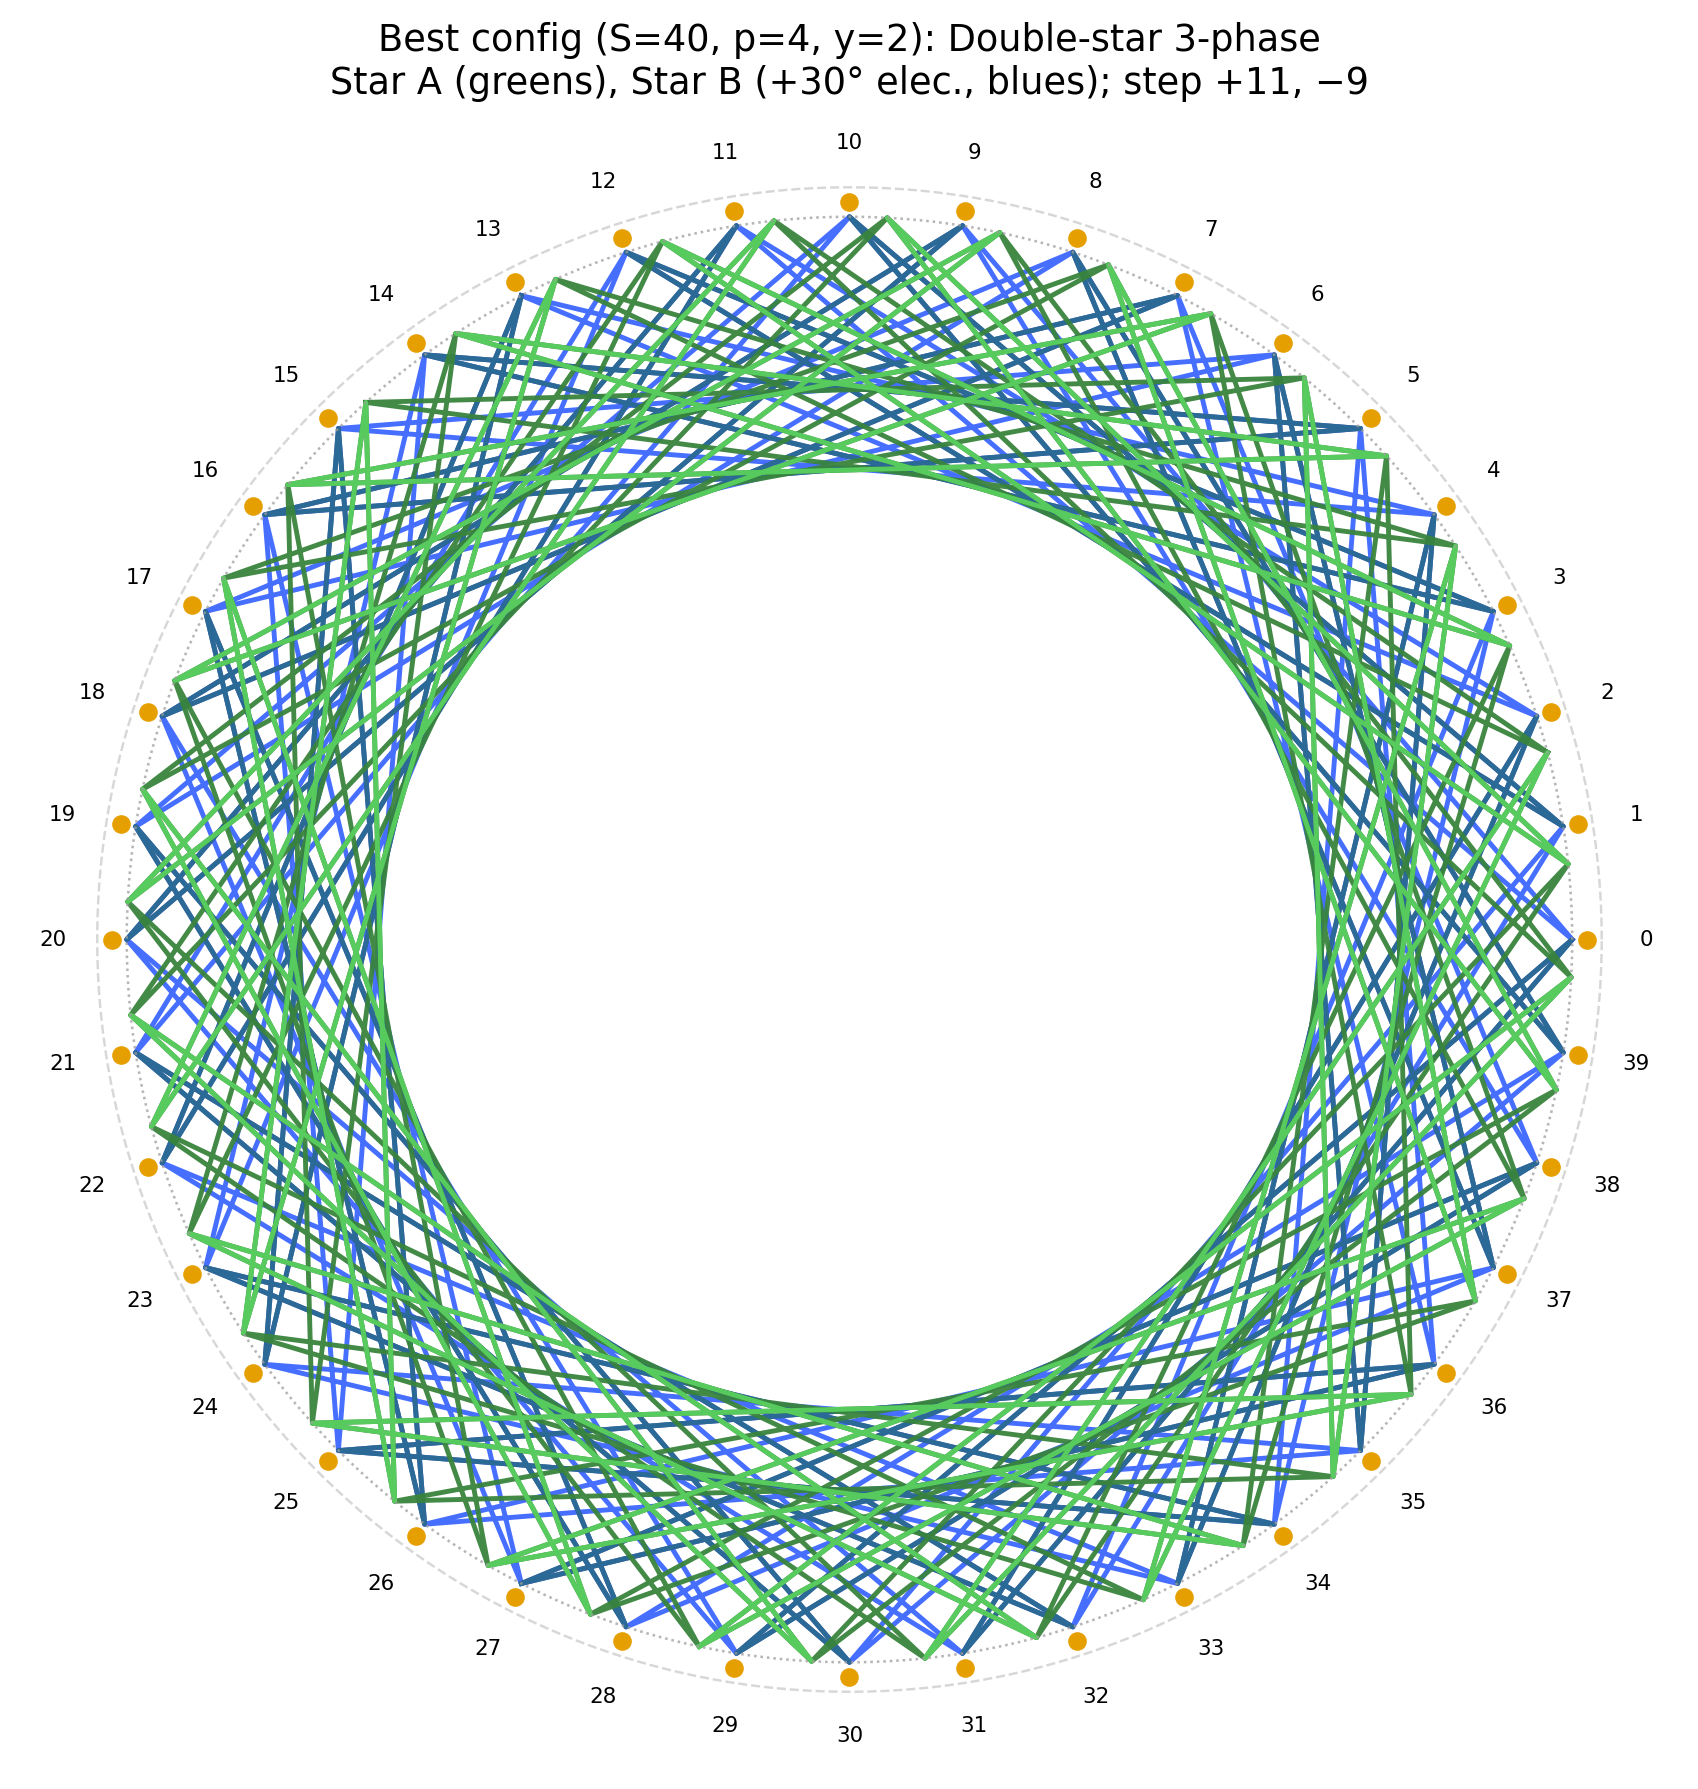
\includegraphics[width=0.7\linewidth]{S40_double_star_best}
        \caption{Double--star 3--phase winding ($S=40$, $p=4$, $y=2$).
        Star~A: greens; Star~B: $+30^\circ$ electrical shift, blues.}
        \label{fig:s40-double-star-best}
        \end{figure}

    \subsection*{Q.2 Stacking (Two Double--Saw-Shapeds)}
        Place two identical Double--Saw-Shaped coils axially stacked (gap $h$).
        Let their on--axis swirl--velocity amplitudes be
        $\mathbf{v}_{\\swirlarrow,T}(z)$ and
        $\mathbf{v}_{\\swirlarrow,B}(z)$.
        Superposition allows the following canonical modes:
        \begin{align*}
        \text{Mode A (additive):}&\quad
        \mathbf{v}_{\\swirlarrow,\text{tot}}\simeq
        \mathbf{v}_{\\swirlarrow,T}
        +\mathbf{v}_{\\swirlarrow,B}
        \quad\Rightarrow\quad
        \text{maximum fundamental amplitude}.\\[3pt]
        \text{Mode B (gradient):}&\quad
        \Delta p =
        \eta\,\tfrac{\rho_{\!f}}{2}
        \big(
        \lVert\mathbf{v}_{\\swirlarrow,B}\rVert^{2}
        -\lVert\mathbf{v}_{\\swirlarrow,T}\rVert^{2}
        \big)
        \quad\Rightarrow\quad
        \text{effective gravity--blocking field}.\\[3pt]
        \text{Mode C (counter--rot.):}&\quad
        \mathbf{v}_{\\swirlarrow,\text{rot}}\!\to 0,\;
        \nabla\lVert\mathbf{v}_{\\swirlarrow}\rVert^{2}\!\neq 0
        \quad\Rightarrow\quad
        \text{standing swirl--pressure pattern}.\\[3pt]
        \text{Mode D (beat):}&\quad
        \varphi\neq 0
        \;\Rightarrow\;
        \text{axially traveling envelope.}
        \end{align*}

    \subsection*{Q.3 Canonical Equation (Swirl Pressure)}
        Within the SST Canon, the swirl pressure on a foliation slice
        $\Sigma_t$ is
        \[
            p_{\mathrm{sw}}(z)
            =\eta\,\frac{\rho_{\!f}}{2}
            \big\langle
            \lVert\mathbf{v}_{\\swirlarrow}(z)\rVert^{2}
            \big\rangle,
        \]
        so that a stacked asymmetry yields the axial force
        \[
            F_z
            =\int_A \Delta p(z)\,dA
            =\eta\,\frac{\rho_{\!f}A}{2}
            \big(
            \lVert\mathbf{v}_{\\swirlarrow,B}\rVert^{2}
            -\lVert\mathbf{v}_{\\swirlarrow,T}\rVert^{2}
            \big).
        \]

        \paragraph*{Rosetta note.}
            Under the Swirl--EM Bridge (Canon~X--XI),
            \[
                B = \sqrt{\tfrac{\rho_{\!f}}{\mu_0}}\,
                \mathbf{v}_{\\swirlarrow},
                \qquad
                \tfrac{B^{2}}{2\mu_0}
                \;\Longleftrightarrow\;
                \tfrac{\rho_{\!f}}{2}
                \lVert\mathbf{v}_{\\swirlarrow}\rVert^{2}.
            \]
            Hence electromagnetic and hydrodynamic forms are equivalent when mapped
            through the canonical density $\rho_{\!f}$.

\subsection*{Q.4 Experimental Pathway}
    \begin{enumerate}
    \item Verify harmonic hygiene: $5^{\mathrm{th}}=0$, $6^{\mathrm{th}}=0$, $7^{\mathrm{th}}\!\ll1$.
    \item Map $\mathbf{v}_{\\swirlarrow}(z)$ or its magnetic proxy $B(z)$ using Hall sensors for both stacks.
    \item Tune $\lVert\mathbf{v}_{\\swirlarrow,B}\rVert /
    \lVert\mathbf{v}_{\\swirlarrow,T}\rVert$ to measure
    $\Delta p$ on a plate of area~$A$.
    \item Switch to Mode~C (counter--rotate top stack) to confirm that
    $\nabla\lVert\mathbf{v}_{\\swirlarrow}\rVert^{2}$
    persists with vanishing torque.
    \end{enumerate}

\subsection*{Q.5 Canonical Status}
    \noindent\textbf{Status: Constitutive Model (Canonical).}
    This configuration is canonical for coil--based RMF realization in SST:
    \begin{itemize}
    \item Implements the harmonic hygiene postulates (Addendum~O).
    \item Realizes swirl--pressure modulation in direct accordance with the
    pressure functional (Canon Core~v0.3.3; Eq.~XVI).
    \item Provides a benchmark experimental platform for
    \emph{gravity--blocking} and pressure--gradient tests.
    \end{itemize}



%================================================
% References
%================================================
\nocite{*}

\bibliography{EM_G}
\bibliographystyle{unsrt}
\end{document}